\documentclass[12pt,letterpaper]{article}
\usepackage[utf8]{inputenc}
\usepackage[spanish]{babel}
\usepackage{graphicx}
\usepackage[left=2cm,right=2cm,top=2cm,bottom=2cm]{geometry}
\usepackage{graphicx} % figuras
% \usepackage{subfigure} % subfiguras
\usepackage{float} % para usar [H]
\usepackage{amsmath}
%\usepackage{txfonts}
\usepackage{stackrel} 
\usepackage{multirow}
\usepackage{enumerate} % enumerados
\renewcommand{\labelitemi}{$-$}
\renewcommand{\labelitemii}{$\cdot$}
% \author{}
% \title{Caratula}
\begin{document}

% Fancy Header and Footer
% \usepackage{fancyhdr}
% \pagestyle{fancy}
% \cfoot{}
% \rfoot{\thepage}
%

% \usepackage[hidelinks]{hyperref} % CREA HYPERVINCULOS EN INDICE

% \author{}
\title{Caratula}

\begin{titlepage}
\begin{center}
\large{UNIVERSIDAD PRIVADA-DE-TACNA}\\
\vspace*{-0.025in}
\begin{figure}[htb]
\begin{center}

\includegraphics[width=8cm]{./Imagenes/logo}
\end{center}
\end{figure}
\vspace*{0.15in}
INGENIERIA DE SISTEMAS  \\

\vspace*{0.5in}
\begin{large}
TITULO:\\
\end{large}

\vspace*{0.1in}
\begin{Large}
\textbf{INFORME DE LABORATORIO No 03} \\
\end{Large}

\vspace*{0.3in}
\begin{Large}
\textbf{CURSO:} \\
\end{Large}

\vspace*{0.1in}
\begin{large}
BASE DE DATOS II\\
\end{large}

\vspace*{0.3in}
\begin{Large}
\textbf{DOCENTE(ING):} \\
\end{Large}

\vspace*{0.1in}
\begin{large}
 Patrick Cuadros Quiroga\\
\end{large}

\vspace*{0.2in}
\vspace*{0.1in}
\begin{large}
Integrantes: \\
\begin{flushleft}
Orlando Antonio Acosta Ortiz		\hfill	(2015052775) \\
Orestes Ramirez Ticona              \hfill  (2015053236) \\
Nilson Laura Atencio     			\hfill 	(2015053846) \\
Roberto Zegarra Reyes 				\hfill 	(2010036175) \\
Richard Cruz Escalante 				\hfill 	(2013047247) \\
\end{flushleft}
\end{large}
\end{center}

\end{titlepage}


\tableofcontents % INDICE
\thispagestyle{empty} % INDICE SIN NUMERO
\newpage
\setcounter{page}{1} % REINICIAR CONTADOR DE PAGINAS DESPUES DEL INDICE

\section{INFORMACIÓN GENERAL} 

\begin{itemize}
\subsection{Objetivos:}
	\item Aplicar y Desarrollar  Consultas con Pivot y Grouping Sets
\subsection{Equipos, materiales, programas y recursos utilizados:}
	\item Microsoft SQL Server 2016, 2017 o superior
	\item Base de datos TSQL
	\item Computadora
	\item Tener una cuenta en Github para subir los cambios


\end{itemize}
\section{MARCO TEORICO} 
\begin{itemize}
\subsection{Base de datos TSQL:}
	\item SQL (Structured Query Language), Lenguaje Estructurado de Consulta es el lenguaje utilizado para definir, controlar y acceder a los datos almacenados en una base de datos relacional.
Como ejemplos de sistemas gestores de bases de datos que utilizan SQL podemos citar DB2, SQL Server, Oracle, MySql, Sybase, PostgreSQL o Access.
El SQL es un lenguaje universal que se emplea en cualquier sistema gestor de bases de datos relacional. Tiene un estándar definido, a partir del cual cada sistema gestor ha desarrollado su versión propia. 
En SQL Server la versión de SQL que se utiliza se llama TRANSACT-SQL.
EL SQL en principio es un lenguaje orientado únicamente a la definición y al acceso a los datos por lo que no se puede considerar como un lenguaje de programación como tal ya que no incluye funcionalidades como son estructuras condicionales, bucles, formateo de la salida, etc. (aunque veremos que esto está evolucionando).
Se puede ejecutar directamente en modo interactivo, pero también se suele emplear embebido en programas escritos en lenguajes de programación convencionales. En estos programas se mezclan las instrucciones del propio lenguaje (denominado anfitrión) con llamadas a procedimientos de acceso a la base de datos que utilizan el SQL como lenguaje de acceso. Como por ejemplo en Visual Basic, Java, C, PHP .NET, etc.

\subsection{Las instrucciones SQL se clasifican según su propósito en tres grupos:}
	\item El DDL (Data Description Language) Lenguaje de Descripción de Datos..
	\item El DCL (Data Control Language) Lenguaje de Control de Datos.
	\item El DML (Data Manipulation Language) Lenguaje de Manipulación de Datos.

\subsection{Consultas con Pivot :}
	\item Las operaciones con Pivot nos permitirá convertir los resultados de una consulta que se presentan en filas y mostrarlos en columnas.
	\item Pivot utiliza las funciones de agregado para presentar los datos en columnas.
	\item El DML (Data Manipulation Language) Lenguaje de Manipulación de Datos.

\subsection{Grouping Sets:}
	\item GROUP BY GROUPING SETS es una poderosa extensión de la cláusula GROUP BY que permite computar múltiples cláusulas de grupo en una sola declaración. El conjunto de grupos es un conjunto de columnas de dimensión.GRUPO POR CONJUNTOS DE GRUPO es equivalente a la UNIONde dos o más operaciones de GRUPO POR en el mismo conjunto de resultados:
	\item GROUP BY GROUPING SETS((a))es equivalente a la operación de conjunto de agrupación única .GROUP BY a
	\item GROUP BY GROUPING SETS((a),(b))es equivalente a .GROUP BY a UNION ALL GROUP BY b
\end{itemize}






\section{PROCEDIMIENTO} 


\begin{enumerate}[1.]
	\item Escribiendo consultas con el operador PIVOT
	\begin{enumerate}[a)]
	\item Task 1: Escribir una sentencia SELECT para recuperar el numero de clientes para un grupo especifico de clientes.\\
		-  Abrir el SQL Server Management Studio y conectar a la basa de datos (local) usando Windows.\\
		-  Usar la base de datos TSQL\\
		-  Ejecutar el siguiente codigo para crear una vista\\
		\begin{figure}[H]
\begin{center}
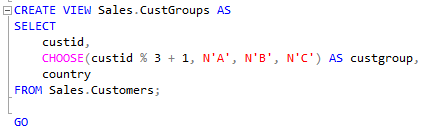
\includegraphics[width=8cm]{./Imagenes/1-1}
\end{center}
\end{figure}
		-  Ejecutar la siguiente consulta
\begin{figure}[H]
\begin{center}
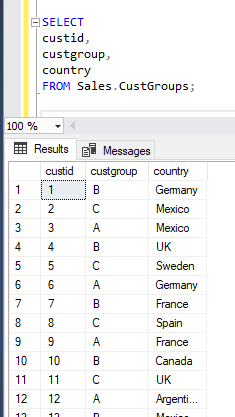
\includegraphics[width=4cm]{./Imagenes/1-2}
\end{center}
\end{figure}
		-  Luego modificamos el codigo, aplicando el operador PIVOT.
\begin{figure}[H]
\begin{center}
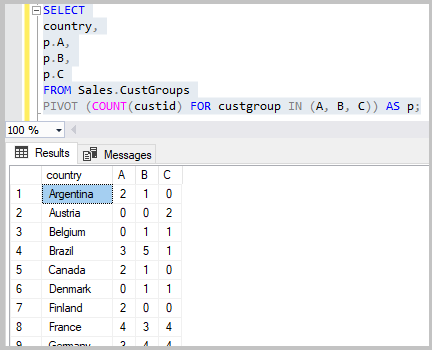
\includegraphics[width=6cm]{./Imagenes/1-3}
\end{center}
\end{figure}
	\item Task 2: Especifique el elemento de agrupacion para el operador PIVOT. \\
		-  Escribir la siguiente consulta y ejecutar. 
		\begin{figure}[H]
		\begin{center}
		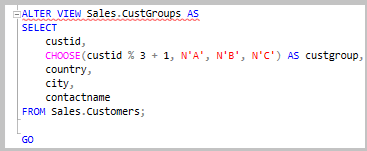
\includegraphics[width=7cm]{./Imagenes/e1-2}
		\end{center}
		\end{figure}
		-  Escribir la siguiente consulta y ejecutar. 
		\begin{figure}[H]
		\begin{center}
		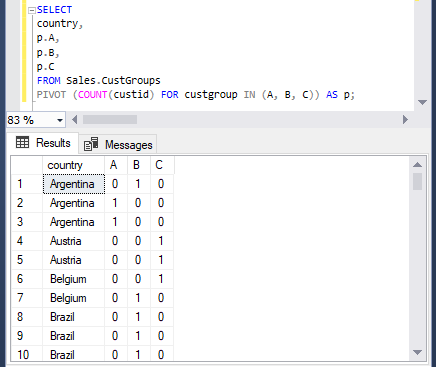
\includegraphics[width=7cm]{./Imagenes/e1-2-1}
		\end{center}
		\end{figure}
		Como se puede observar tiene el mismo resultado que en la consulta de Task1
		-  Modificar la consulta para incluir columnas adicionales desde la vista y ejecutar. 
		\begin{figure}[H]
		\begin{center}
		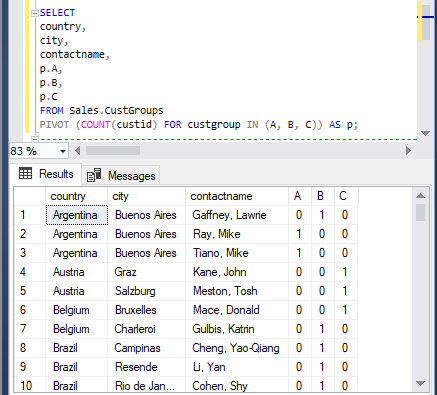
\includegraphics[width=7cm]{./Imagenes/e1-2-2}
		\end{center}
		\end{figure}
		Como se puede observar tiene el mismo resultado que en la consulta de Task1
	\item Task 3: Use una expresion de tabla común (CTE) para especificar el elemnto de agrupacion para el operador PIVOT.\\
		-  Escribir la siguiente consulta y ejecutar. 
		\begin{figure}[H]
		\begin{center}
		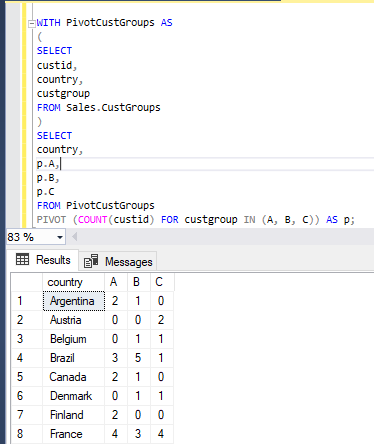
\includegraphics[width=7cm]{./Imagenes/3-1}
		\end{center}
		\end{figure}
		Como se puede observar tiene el mismo resultado que en la consulta de Task1
	\item Task 4: Escribe una instruccion SELECT para recuperar el monto total de ventas para cada cliente y categoria de producto.\\
		-  Escribir la siguiente consulta y ejecutar. 
		\begin{figure}[H]
		\begin{center}
		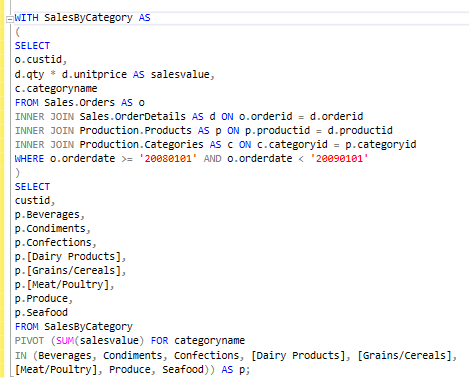
\includegraphics[width=8cm]{./Imagenes/3-2}\\
		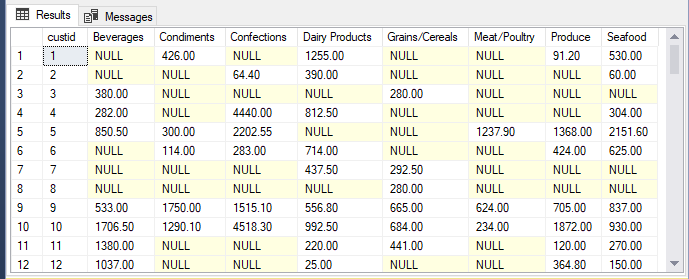
\includegraphics[width=8cm]{./Imagenes/3-3}
		\end{center}
		\end{figure}
	\end{enumerate}

	\item Escribiendo consultas con el operador UNPIVOT
	\begin{enumerate}[a)]
	\item Task 1: Crear y consultar la vista Sale.PivotCustGroups.\\
		-  Escribir la siguiente consulta y ejecutar para crear una vista llamada Sales.PivotCustGroups.\\
		\begin{figure}[H]
		\begin{center}
		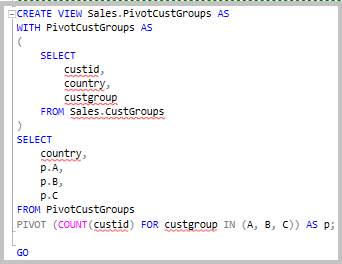
\includegraphics[width=8cm]{./Imagenes/e2-1}
		\end{center}
		\end{figure}
		-  Despues escribrir y ejecutar la siguiente consulta.
		\begin{figure}[H]
		\begin{center}
		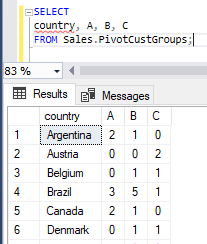
\includegraphics[width=6cm]{./Imagenes/e1-1-1}
		\end{center}
		\end{figure}
	\item Task 2: Escriba una instruccion SELECT para recuperar una fila para cada pais y grupo de cliente.\\
		-  Escribir la siguiente consulta y ejecutar.\\
		\begin{figure}[H]
		\begin{center}
		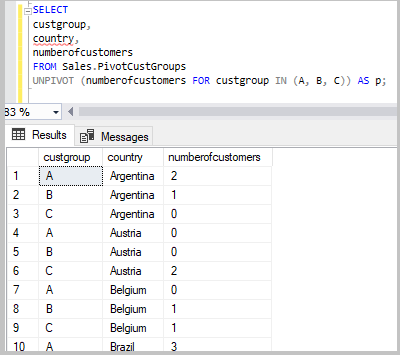
\includegraphics[width=8cm]{./Imagenes/e2-2}
		\end{center}
		\end{figure}
	\item Task 3: Eliminar las vistas creadas.
		\begin{figure}[H]
		\begin{center}
		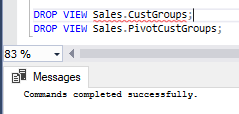
\includegraphics[width=6cm]{./Imagenes/e2-3}
		\end{center}
		\end{figure}
	\end{enumerate}



	\item Escribiendo consultas con las clausulas GROUPING SETS, CUBE, and ROLLUP.
	\begin{enumerate}[a)]
	\item Task 1: Escriba una instruccion SELECT que use LA SUBCLAUSULA GROUPING SETS para devolver el número de
Clientes para diferentes conjuntos de agrupación.\\
		-  Escribir la siguiente consulta y ejecutar. 
		\begin{figure}[H]
		\begin{center}
		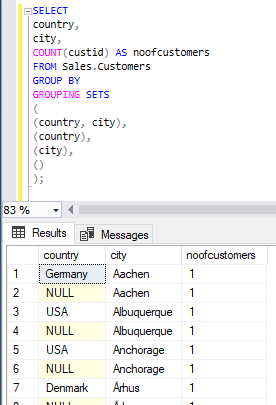
\includegraphics[width=7cm]{./Imagenes/e3-1}
		\end{center}
		\end{figure}
	\item Task 2: Escriba una instruccion SELECT que use la subclausula CUBE para recuperar Grouping sets basados en valores de ventas anuales, mensuales y diarios.\\
		-  Escribir la siguiente consulta y ejecutar. 
		\begin{figure}[H]
		\begin{center}
		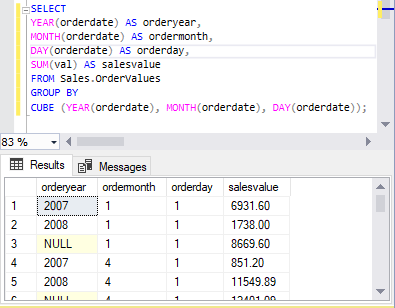
\includegraphics[width=7cm]{./Imagenes/e3-2}
		\end{center}
		\end{figure}
	\item Task 3: Escriba la misma instruccion SELECT usando la cubclausula ROLLUP.\\
		-  Escribir la siguiente consulta y ejecutar. 
		\begin{figure}[H]
		\begin{center}
		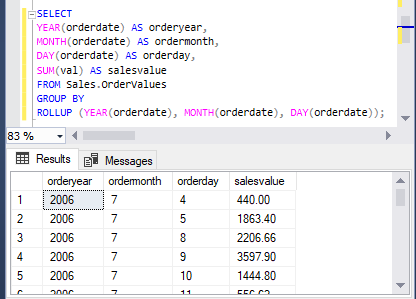
\includegraphics[width=7cm]{./Imagenes/e3-3}
		\end{center}
		\end{figure}
	\item Task 4: Analizar el valor total de ventas por año y mes.\\
		-  Escribir la siguiente consulta y ejecutar. 
		\begin{figure}[H]
		\begin{center}
		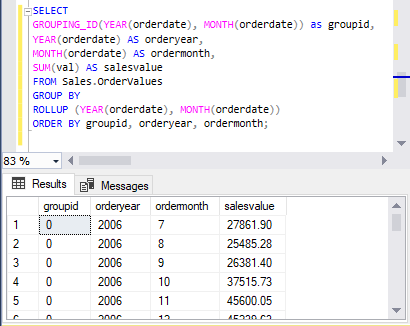
\includegraphics[width=7cm]{./Imagenes/e3-4}
		\end{center}
		\end{figure}
	\end{enumerate}
\end{enumerate}




\section{ANALISIS E INTERPRETACION DE RESULTADOS} 

\section{CONCLUSIONES}
\begin{itemize}
	\item Durante el desarrolo del laboratorio se puso en practica todo sobre el uso del T-SQL para realizar el cambio de filas a columnas. Una de estas opciones fue el PIVOT que importante y simple que nos permite, en lugar de crear un codigo complejo, un código con referencias cruzadas a partir de cualquier tabla.
	\item Con PIVOT podemos cambiar la orientación de la tabla hasta visualizar los datos de forma que le sea más útil y fácil el análisis. Cambiar la orientación permite examinar las secciones cruzadas seleccionadas de datos.
\end{itemize}


\section{REFERENCIAS} 


\end{document}
